%% LaTeX template for BSc Computing for Games final year project dissertations
%% by Edward Powley
%% Games Academy, Falmouth University, UK

%% Based on:
%% bare_jrnl.tex
%% V1.4b
%% 2015/08/26
%% by Michael Shell
%% see http://www.michaelshell.org/
%% for current contact information.
%%
%% This is a skeleton file demonstrating the use of IEEEtran.cls
%% (requires IEEEtran.cls version 1.8b or later) with an IEEE
%% journal paper.
%%
%% Support sites:
%% http://www.michaelshell.org/tex/ieeetran/
%% http://www.ctan.org/pkg/ieeetran
%% and
%% http://www.ieee.org/

%%*************************************************************************
%% Legal Notice:
%% This code is offered as-is without any warranty either expressed or
%% implied; without even the implied warranty of MERCHANTABILITY or
%% FITNESS FOR A PARTICULAR PURPOSE! 
%% User assumes all risk.
%% In no event shall the IEEE or any contributor to this code be liable for
%% any damages or losses, including, but not limited to, incidental,
%% consequential, or any other damages, resulting from the use or misuse
%% of any information contained here.
%%
%% All comments are the opinions of their respective authors and are not
%% necessarily endorsed by the IEEE.
%%
%% This work is distributed under the LaTeX Project Public License (LPPL)
%% ( http://www.latex-project.org/ ) version 1.3, and may be freely used,
%% distributed and modified. A copy of the LPPL, version 1.3, is included
%% in the base LaTeX documentation of all distributions of LaTeX released
%% 2003/12/01 or later.
%% Retain all contribution notices and credits.
%% ** Modified files should be clearly indicated as such, including  **
%% ** renaming them and changing author support contact information. **
%%*************************************************************************


\documentclass[journal]{IEEEtran}

\usepackage{graphicx}
\usepackage[utf8]{inputenc}
\usepackage{url}
\usepackage{amsmath}
\usepackage[]{algorithm2e}
% Insert additional usepackage commands here

\begin{document}
%
% paper title
% Titles are generally capitalized except for words such as a, an, and, as,
% at, but, by, for, in, nor, of, on, or, the, to and up, which are usually
% not capitalized unless they are the first or last word of the title.
% Linebreaks \\ can be used within to get better formatting as desired.
% Do not put math or special symbols in the title.
\title{Extending Client Side Prediction Methods in Networked Multiplayer First Person Shooter Games to Include Level Information}
%
%
% author name
\author{Richard Steele}

% The paper headers -- please do not change these, but uncomment one of them as appropriate
% Uncomment this one for COMP320
\markboth{COMP320: Research Review and Proposal}{COMP320: Research Review and Proposal}
% Uncomment this one for COMP360
% \markboth{COMP360: Dissertation}{COMP360: Dissertation}

% make the title area
\maketitle

% As a general rule, do not put math, special symbols or citations
% in the abstract or keywords.
\begin{abstract}
This paper critically examines the effectiveness of the current methods of client side prediction in networked multiplayer digital games, specifically first person shooter games where the accuracy of each game agent's behaviour is critical to the player's experience. The de facto use of \textit{dead reckoning} is accepted as a standard tool to help minimise the number of required network updates, but its results can be error prone which are a detriment to the player's experience. This paper looks at the currently used dead reckoning algorithms and suggests using further data about the game state to provide a more accurate estimation of a game agent's location and behaviour at a future time. Information regarding the layout of a level is used influence acceleration factor in the dead reckoning algorithm and to dynamically alter the allowance threshold to better reflect an agent's behaviour at critical locations in the level by prompting an increased rate of player state updates.
\end{abstract}

\section{Introduction}
% The very first letter is a 2 line initial drop letter followed
% by the rest of the first word in caps.
% 
% form to use if the first word consists of a single letter:
% \IEEEPARstart{A}{demo} file is ....
% 
% form to use if you need the single drop letter followed by
% normal text (unknown if ever used by the IEEE):
% \IEEEPARstart{A}{}demo file is ....
% 
% Some journals put the first two words in caps:
% \IEEEPARstart{T}{his demo} file is ....

\IEEEPARstart{W}{ith} modern networked multiplayer digital games where the game state must be updated often, it is impractical to send and receive network updates on every frame. Instead, \textit{dead reckoning} algorithms are used to predict future states of the game, and network updates are needed only when the actual behaviour differs from the predicted behaviour by a threshold amount. This idea of an acceptance threshold accepts that the perception of an entity for all other clients on a network may differ to the actual state of that entity. While effective at greatly reducing the required network updates and reducing the impact of network transmission delay \cite{pantel2002suitability}, impossible behaviours such as tunnelling (projecting a position past a barrier), or improbable behaviours counter intuitive to the game are possible. This paper proposes that by using further information about the game state, such as level layout, an agent's behaviour can be predicted with greater accuracy to help minimise unwanted behaviour.

Previous papers in the context of games describe dead reckoning as a measure to account for network latency compensation. Few expand beyond this and are concerned generally with how best to marry the predicted state with the actual state by interpolation or rolling back. This paper explores improving the accuracy of the simulation by dynamically adjusting the threshold allowed by traditional dead reckoning methods to prompt more frequent state updates at critical times when the greatest accuracy is required.
% It should be noted that not all networked multiplayer games suffer from latency problems. 
%It is important to note that not all networked multiplayer games suffer from client side prediction problems.

It should be noted that not all networked multiplayer games suffer from latency problems. For instance turn based games consider each client sequentially. Where there is no scope or benefit for a player to react immediately, no measures must be taken to account for problems incurred by some milliseconds lost in transmission. These issues are prevalent in fast paced competitive games such as racing games, or the first person shooter genre. This paper then bases its study upon the first person shooter game genre, sometimes referred to as \textit{twitch} shooters \cite{lee2015outatime}. The need to respond quickly to other clients' perceived actions is critical to the player experience, therefore it is crucial that those actions are shown as accurately as possible.

The research question that this paper addresses is: how can client side prediction in networked multiplayer first-person shooter games that use dead reckoning be improved?

\section{Background}

This literature review first confirms the definition of client side prediction, the problems that it solves, and the trade off against absolute accuracy. Dead reckoning is explained and explored with a focus on the real world applications and techniques of its use within games. Finally, alternative methods of solving the the problems associated with network latency are explained and acknowledged.

\subsection{Client side prediction}

Networked multiplayer games are defined as sharing a game space between multiple clients \cite{diot1999distributed}. Each client holds a representation of that game space which it uses to display information to the user, and allows the user to change within the rules of the game. When elements or details of the agents of that game space are changed by a client's actions, the client assumes that the action is successful, performs that action on its own game state representation, then sends the action information to the network so as all other clients can update their own game space representation to reflect the performed action \cite{bernier2001latency}.

Problems can occur when:
\begin{itemize}
    \item the updated information is received too late (network latency)
    \item the updated information is not received (packet loss)
    \item the action is not successful (simultaneous conflicting actions are performed by many clients).
\end{itemize}

Network latency forms the primary bottleneck for online game performance with an acceptable value being under 100 milliseconds \cite{lee2015outatime} \cite{smed2002aspects} and worst case overall latencies claimed to be up over 1 second \cite{claypool2006latency}. To counter this, each client takes the slightly old network state update that it receives and brings it approximately up to date through extrapolation before displaying it to the user. Performance degrades significantly under variance in latency (or \textit{Jitter}) \cite{beigbeder2004effects} \cite{dick2005analysis}. The jitter effect must be continually accounted for as the delta time value between updates can be subject to change. As such, the current time in which an action is performed is included with the update packet of data sent and received by clients, and forms an integral part of the prediction algorithm. The latency time difference must be continuously evaluated by sending and receiving time stamped packets to maintain a correct delta time value \cite{glazer2015multiplayer}, however manipulating these time stamps is an opportunity for cheating \cite{jamin2003cheat} so must be secure from interference or if using a centralised server then a globally synchronised clock can be used \cite{aggarwal2004accuracy}.

Given the vast quantity and unreliable nature of the messages being sent \cite{cronin2001distributed}, packet loss must be planned for. The same dead reckoning methods used to account for network latency, and outlined in \textit{B.} can be used to replace missing packets of information, or application data units (ADUs) \cite{diot1999distributed} sometimes referred to as protocol data units (PDUs) \cite{dis1998ieee}, to supply a prediction of where the ADU's agent will ``most probably'' be at a given time.

\subsection{Dead reckoning}

Dead reckoning methods are based on a navigational technique of estimating one’s position based on a known starting point and velocity \cite{smed2002aspects}. In the simplest implementation, we take the last position we received on the network, and project it forward in time with at its last known velocity \cite{murphy2011believable}.

\begin{figure}[h]
    \centering
    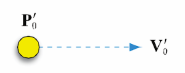
\includegraphics[width=0.3\linewidth]{DR1.png}
    \caption{First order linear projection. Image sourced from \cite{murphy2011believable}}
    \label{fig:dr1}
\end{figure}

This simple representation of projecting forward is correct if an agent has linear movement and constant velocity. However, agents in a first person shooter game often have complex non linear movements which will need to be checked for and accommodated. Real world applications of linear dead reckoning also suffer with having to account for unpredictable behaviour e.g. drift due to wind or wheel slippage \cite{chung2001accurate} \cite{ojeda2004experimental}. The techniques used for managing these behaviours are transferable to the problems of dead reckoning networked multiplayer game agents with complex behaviour.

In 1983, with substantial support from the U.S. army, the Defense Advanced Research Projects Agency (DARPA) initiated the Simulator Networking (SIMNET) program which developed dead reckoning techniques to support a virtual world to train soldiers \cite{calvin1993simnet}. Their approach to networking solutions has been incorporated into the Distributed Interactive Simulation (DIS) standard which is now an IEEE standard \cite{dis1998ieee}. It outlines the use of a PDU to help dead reckoning handle complex behaviour \cite{mccarty1994virtual}. It is worth remembering however that DIS was designed for use by a small number of players (less than 50), and the inclusive PDU model can be criticised for holding too much redundant data \cite{henderson2001latency}.
 
Each client maintains a dead reckoned model of itself that corresponds to the model used by other clients to ``see'' its represented agent. The client must regularly check whether the difference between the predicted state calculated with dead reckoning that all clients share and the actual state exceeds a certain threshold. If this is the case, the client is then responsible to generate an updated entity state for the dead reckoning algorithm to apply to the model. Then send that updated state to all clients on the network to learn about the correct new state of the entity to then use to update their own model of that client's agent \cite{calvin1993simnet} \cite{mauve2000keep}. This also happens when a fixed amount of time has passed since the last update (normally 5 seconds) \cite{mills1992network}.

\begin{figure}[h]
    \centering
    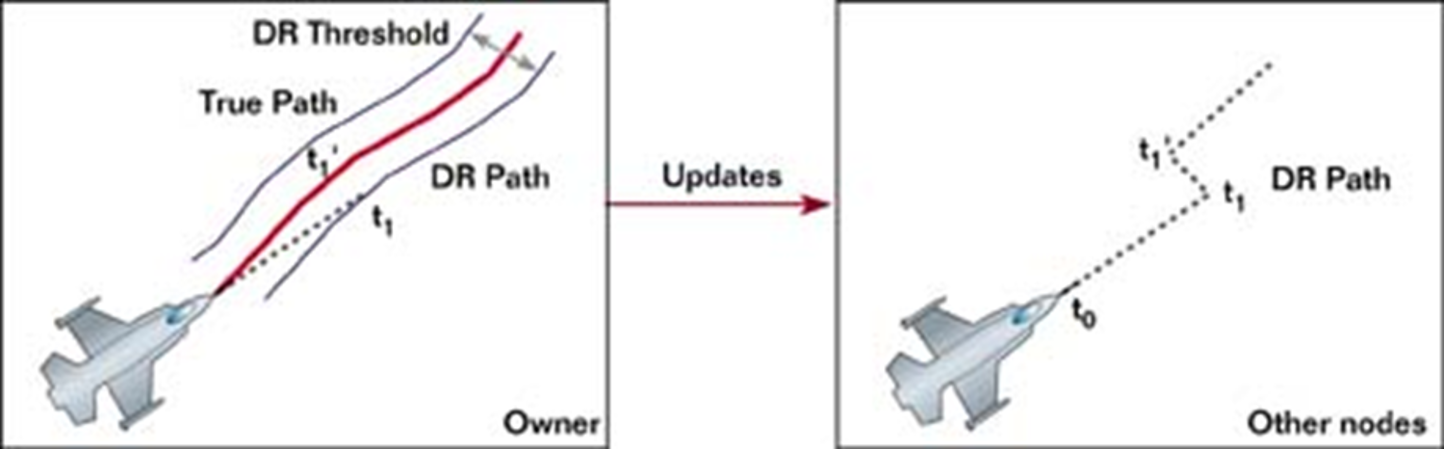
\includegraphics[width=0.8\linewidth]{Threshold1.png}
    \caption{Image sourced from \cite{aronson1997gamasutra}}
    \label{fig:threshold}
\end{figure}

Were this updated information used immediately, the modelled entity would appear to jump (fig. \ref{fig:threshold}). Instead, the dead reckoning algorithm uses interpolation and projective velocity blending \cite{murphy2011believable} to tend towards and eventually reconcile its own dead reckoned model with the updated state information.

\begin{figure}[h]
    \centering
    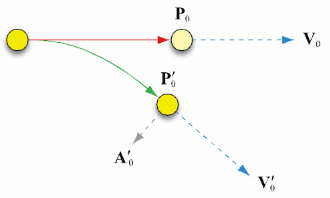
\includegraphics[width=0.7\linewidth]{DR2.png}
    \caption{Upon update, the difference between the simulation shown in red and the actual position shown in green is observed. Image sourced from \cite{murphy2011believable}.}
    \label{fig:dr2}
\end{figure}

\begin{figure}[h]
    \centering
    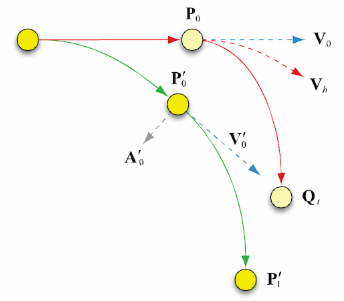
\includegraphics[width=0.7\linewidth]{DR3.png}
    \caption{With interpolation the simulation attempts to reconcile itself with the updated position and motion as explained in section C. Image sourced from \cite{murphy2011believable}.}
    \label{fig:dr3}
\end{figure}

\subsection{Implementation}

Reconciling deviations with projective velocity blending

\begin{align}
        Q_t & = P_0 + VT \\
        Q_t & = {P'_0} + {V'_0} T + \frac{1}{2} {A'_0} T^2 \\
        V_b & = V_0 + ({V'_0} - {V_0}) \Hat{T}  \\
        P_t & = P_0 + {V_b}{T_t} + \frac{1}{2} {A'_0} {T_t^2}  \\
        P'_t & = {P'_0} + {V'_0}{T_t} + \frac{1}{2}{A'_0}{T_t^2}\\
        Q_t & = P_t + ({P'_t} - P_t ) \Hat{T} 
\end{align}

Where $Q_t$ is the dead reckoned position at a specific time $T$ for an entity starting at position $P$, moving at velocity $V$, with acceleration $A$. As shown in fig \ref{fig:dr2} and fig \ref{fig:dr3}, prime ($'$) refers to the actual entity rather than the simulated model. The subscript $0$ refers to the starting value, subscript $t$ is that value at time $T$, and subscript $b$ is the blended model between actual and simulation values.
\\ \\
(1) First order linear projection. Shown in fig \ref{fig:dr1} as projecting a velocity over time from a position.\\
(2) Second order projection adds the derivative of acceleration applied according to Newton's laws of motion.\\
(3) Shows a velocity blending model given two velocities. In client side prediction this would be the simulated velocity and the actual velocity. $V_b$ will tend towards the actual velocity $V'_0$ as delta time $\Hat{T}$ tends towards $1$. \\
(4) Applies the blended velocity value with the simulation's starting position to the second order projection in (2) giving the simulated position at time $T$.\\
(5) Applies the last known actual values to the second order projection in (2) giving the updated projection position at time $T$.\\
(6) Blends these positions tending the simulation towards the updated projection position as delta time $\Hat{T}$ tends towards $1$.

\hrulefill

{\sc Threshold based dead reckoning pseudo code}

\hrulefill

\begin{algorithm}
\DontPrintSemicolon % Some LaTeX compilers require you to use \dontprintsemicolon instead
\KwIn{ \\ prediction error threshold: $\eta$ \\ time at which the last position was sent: $t_o$ \\ actual position (at time $t$): $x_t$}
%$t_0 \gets -\infty$\;
\ForEach{frame (time $t$)}{
  $\Hat{x}_t \gets$ prediction($x_{t_0}, t$);\;
    \If{$||x_t - \Hat{x}_t|| > \eta $}{
        send update packet(x_t)\\
        $t_0 \gets t$\;
    }
}
\caption{A client predicts the position of their own agent for the current frame based on the last sent position update. If the prediction error is larger than the threshold ${\eta}$ then an update packet is sent to the network and the simulation resets itself.}
\label{algo:pseudo}
\end{algorithm}

\subsection{Interest modelling}

The shortcomings of estimating a game agent's behaviour based solely upon motion dynamics are already recognised and attempts to address these problems with further information have been somewhat explored. The \textit{Donnybrook} protocol \cite{bharambe2008donnybrook} looks to increase the delay between packets up to seconds by leveraging human cognitive limitations to preferentially spend bandwidth capacity on information most important to the player's \textit{interest sets}. Similarly, Amir Yahyavi \textit{et al} successfully use identified points of interest to influence their dead reckoning algorithm, improving the accuracy by up to 30\% over traditional dead reckoning techniques \cite{yahyavi2011antreckoning}.

Yahyavi \textit{et al} propose the use of \textit{attraction forces}, derived from the player state and nearby points of interest, to be factored into the dead reckoning calculation alongside the current acceleration. The example that they often cite states that a player controlling an entity with reduced health will most likely move towards a health pack if there is one in sight. However, their method titled \textit{AntReckoning} must decide on the attraction forces of each point of interest, to build a \textit{pheromone map}. AntReckoning's weakness is great complexity as every change in the game state affects nearby attraction forces. Also the reliability of AntReckoning can be disputed as different players may have differing goals, but the increase in accuracy reported is excellent. This can also be used to influence the path finding algorithms of non playable characters (NPCs) controlled by an artificial intelligence to direct them towards popular parts of the level \cite{yahyavi2013interest} \cite{yahyavi2013towards}. While this shows an interesting application of utilising level information, the behaviour of NPCs is beyond the scope and focus of this project.



The merit of Amir Yahyavi \textit{et al}'s work \cite{yahyavi2011antreckoning} \cite{yahyavi2013interest} recognising and proposing solutions to the problems of solely using traditional dead reckoning methods in games with client side prediction is acknowledged, and an inspiration for this project.

\subsection{Adapting the acceptance threshold}

As shown in algorithm \ref{algo:pseudo}, the condition that prompts a network update is that the difference in position between a client's own entity and the representation of that entity used by the network differ by more than a threshold amount. This amount can be visualised as an acceptance radius around the dead reckoned position as shown in fig \ref{fig:threshold}. Generally, dead reckoning algorithms employ a fixed threshold \cite{cai1999auto}. Related work that investigates changing this threshold amount depending on game state conditions decide the variance by considering the individual peer to peer relationships such as the distance between the entities. This \textit{relevance filtering} is reliant upon a \textit{radius of interest} \cite{rak1996evaluation}. The reasoning given is that distant entities are not likely to interact with each other so accuracy is not extremely important  \cite{cai1999auto} \cite{jaya2016combining}.

This paper acknowledges this method's effectiveness in specific situations to reduce network updates. But, given the often edge to edge viewing range prevalent in many game first person shooter levels \cite{toby2014tobyscs} \cite{ziervogel2014nag} \cite{cod2018wikibo4}, this paper argues against its use in a general approach to improving client side prediction in first person shooter games.

To allow for edge to edge sight lines and the prevalent long range weapons available for use in first person shooter games, we can consider filtering for entities that are within that player’s potential field of sight \cite{cronin2001distributed}. However, this requires previous knowledge of all entity positions therefore a two pass approach would be needed to determine which entities would be affected by a state change, and then to update those clients. Also, care must be taken as even when entities are out of sight of each other, dead reckoning may predict a behaviour which results in the entities being revealed and the integrity of the game state will be compromised.

Roberts \textit{et al.} propose that network update time should be factored into deciding the threshold limit value. Network limitations when presented with a large amount of packets may result in inconsistency for which additional updates are needed to rectify \cite{roberts2008bounding}. This shortcoming in a networked application is an important consideration. However, given the local prediction methods of this project, fall outside of this study. Were future work to lead to a networked experiment, and given the proposed increase in packets sent at critical junctures, the relevance of considering network shortfalls when calculating a dynamically changing threshold will be crucial.



% Read the threshold adapting papers then write up that bit
% Same for the Heat maps
% Methodology

\subsection{Doppelg\"{a}ngers}

\textit{Doppelg\"{a}ngers} offer a promising alternative that will adhere to the game's rules and avoid impossible behaviour. Jeffrey Pang \textit{et al.} discuss populating a client's game state representation with computer-controlled players known as \textit{bots}. Updates prompted by a threshold based system similar to that outlined in algorithm \ref{algo:pseudo} will contain \textit{guidance} for the artificial intelligence (AI) to rectify and better replicate the relevant representation \cite{pang2007scaling} \cite{bharambe2008donnybrook}. As most first person shooter games contain AI routines for single player modes, much of the work needed to guide a bot around a level has been done. Problems will occur if a bot representation decides that it will perform an action such as shoot at an enemy, whereas the actual behaviour does not. Questions arise such as should the bot then fire ``blanks'', and consideration must be given as to whether that action may inadvertently alert enemies to that entity's position? This approach shows considerable potential in providing possible and realistic representations of other clients' behaviours, but relies heavily upon accurately portraying and dynamically adjusting the player's behaviour model. To configure the AI behaviour, neural networks can be trained and used to predict changes of the entity velocity \cite{mccoy2007multistep}. Jeffrey Pang \textit{et al.} propose that a blending between an AI bot for non-critical behaviour e.g. outside of the client's focus, and conventional dead reckoning state updates for representations of entities within the player's focus will provide a satisfying result \cite{pang2007scaling}.

This paper argues in favour of bot representations as both a method to decrease the frequency of network updates, and as a tool to extrapolate future behaviours. But, also acknowledges its dependency upon accurate player modelling techniques. Player modelling is an ongoing study in the field of games. Since the focus of this work is on dead reckoning in client side prediction we omit further details about AI modelling player behaviour, although we strongly consider this as future work in the field of client side prediction.

\section{Discussion}

The two part purpose of client side prediction is to maintain an up to date game state for clients in the case of late or lost packets, and to use prediction algorithms to reduce required network updates. While the simplest dead reckoning algorithm provides a linear vector approximation based on velocity, we have shown above that interpolation and projective velocity blending can be used to smooth trajectories between state updates tending towards the correct representation.

Benjamin Kuipars states that the difficulty of a dead reckoning task should vary according to the number of turns in the route, while the error rate and magnitude should vary according to the departure from straight \cite{kuipers1978modeling}. So, we can infer that likewise when considering complex paths with many turns, to expect a larger error rate.

It is a fundamental requirement for believable games that the state transitions and corrections are smooth and believable, shown in figures as a curve tending towards the target rather than a jump. These curves are shown to be accurate when inferred from polynomial modelling based on the Lagrange or Taylor series \cite{hanawa2006proposal}. But require multiple states from which to extrapolate an approximation. Packet loss can be greatly detrimental to this approach. Small sample sizes combined with potentially erratic movement of game players will likely produce unlikely results. A solution would be to provide back up copies of previous states in each PDU to restore missing information. A technique already employed in Quake where the last three commands are also sent in each packet to compensate for lost packets \cite{cronin2001distributed}. James M. Van Verth and Lars M. Bishop provide a method to sample and project cubic bezier spline curves \cite{van2008essential} but these are shown to be slightly less accurate than the velocity blending technique shown above proposed by Curtiss Murphy \cite{murphy2011believable}. 

Dead reckoning is an \textit{optimistic algorithm}. It assumes it is correct  and when it is not, it must adjust itself. It is apparent that the blending of this adjustment may result in compromising behaviour. Demonstrated in first person shooter games as appearing to other players in a vulnerable position outside of cover, or moving through an impenetrable area as defined by the game's movement rules. Consider the velocity blending method shown in fig \ref{fig:dr3} and (6). A player could turn instantaneously and the algorithm would apply unrealistic forces to create huge accelerations at arbitrary angles \cite{bernier2001latency}. Large inconsistencies due to extremely late updates may even lead to repairs requiring a state rollback which will cause more drastic position jumps \cite{cronin2002efficient}. The resulting movement shown by the red line in fig \ref{fig:dr3} may fall outside the rules of the game. Either passing through untraversable locations such as through walls or over gaps, or into unlikely locations according to the game's rules such as into a vulnerable position outside of cover. Many networked multiplayer first person shooter games suffer from criticism because of this. Players can feel unfairly treated and forums discussing these issues become very popular with many thousands of views \cite{rout2013youtube} \cite{gkac2014gamefaqs} \cite{drift0r2013youtube} \cite{solaire2016reddit} \cite{ss2018reddit} \cite{hp2015bungie}.

The de facto method of dead reckoning entities' behaviours is a distributed approach that does not require a centralised server. Using a distributed approach is mandatory for many distributed virtual environments (DVEs) in order to avoid the well known problems of centralised systems such as increased latency, single-point-of-failure and lack of scalability \cite{mauve2000keep}. However, having a dedicated central authoritative server (or a single client nominated as such) means that if a client simulates different results than the server, the server’s results will eventually correct the client’s incorrect simulation \cite{bernier2001latency}.

Laurent Gautier and Christophe Diot propose that late packets due to network latency may be accommodated by the client by introducing a local presentation delay to provide a consistent, distributed state \cite{gautier1998design}. Trailing state synchronisation is designed specifically for real-time multiplayer games, and achieves better responsiveness and scalability while maintaining near-perfect consistency \cite{cronin2001distributed}. However, these increase the application-level delay even more so. While this method termed \textit{time warp} is acceptable for their MiMaze maze navigation project, it is unsuitable for the fast paced style of first person shooter games.

In the interest of completeness, in $II.A.$ we mention network latency not succeeding due to a state conflict, where simultaneous conflicting actions are performed by multiple clients. In this case, the authoritative server, the client acting as such, or the game itself, must decide which state is the ``correct'' state and update all conflicting clients with the decision. Games will often invoke a small delay before critical moments e.g. a death animation, to allow conflicting states to resolve themselves before committing to a particular irreversible state. With this delay, the game can rollback to the correct state without the user experiencing a jarring state change \cite{mauve2000keep}.

\subsection{Representing level data}

This project proposes that information pertinent to the level layout can be used to better predict an agent's behaviour, and more critically evaluate when to send update packets. As such, effectively storing and evaluating spatial information about the changes in motion of agents moving around a level is paramount. 

A heat map is a visual reflection of a statistical model \cite{wilkinson2009history} used often in games to graphically represent spatial analytics of player telemetry with colours, overlayed upon a traditional map of the level (see fig \ref{fig:hm1}). They are a tool to help extract patterns and knowledge which can be used to detect outlying data \cite{drachen2013spatial} (Apparent in fig \ref{fig:hm3} as single paths travelling perpendicular to the trend). To this end, as a tool, it meets our needs perfectly. Where interest modelling seeks to better predict a single entity's interest,
our proposed method outlines a broadly applicable standard per level by using irrefutable information about the level to better avoid dead reckoning projecting a client's position into an unlikely or impossible location.

Heat maps are used in games for training bots to behave more realistically and improve map design during development \cite{bauckhage2014beyond} but to the best of our knowledge has not been applied to alter attraction forces in dead reckoning algorithms or alter the network update frequency.

Unlike the path visualisation as shown in fig \ref{fig:hm2}, the direction of motion must be asymmetric. Consider that a player may jump down from a platform but be unable to get back onto it \cite{bauckhage2014beyond}. The data must also be stored as such that symmetric paths such as corridors must preserve a direction vector, so as opposite paths do not cumalate to a zero score. Our method relies on the idea that a perpendicular vector to the trend must be realised as countering the norm.

Finally, the map must be partitioned in such a way that the information is relevant. Equal size cell partitioning can disproportionately accumulate several critical positions within, while other less dense cells may merely be a space of travel between key junctures \cite{steed2003partitioning}. It is impossible to declare equally important cell boundaries before collecting some data on the level so this project must rely upon extracting and analysing level data before formatting it into a state that the client side prediction algorithms can effectively use.

\begin{figure}[h]
    \centering
    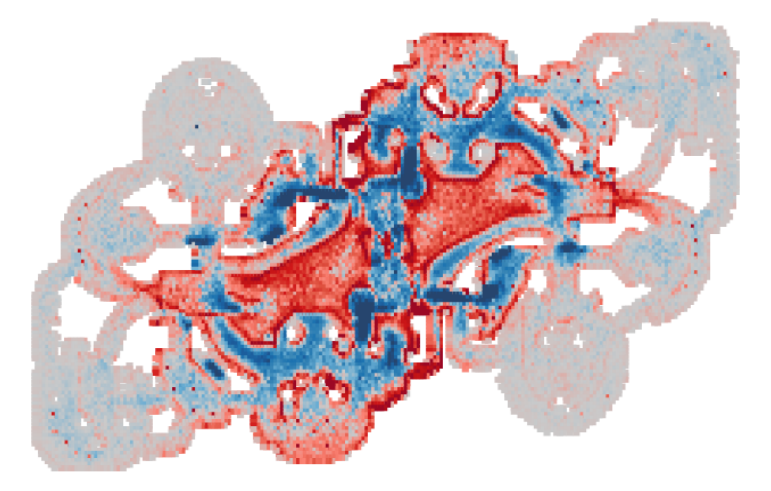
\includegraphics[width=0.9\linewidth]{Heatmap1.png}
    \caption{Example of overlay analysis. A balance heatmap from the ``Molten'' map from the game \textit{Transformers: War for Cybertron}. Red areas indicate deaths and blue areas indicate kills. Image sourced from \cite{drachen2013spatial}.}
    \label{fig:hm1}
\end{figure}

\begin{figure}[h]
    \centering
    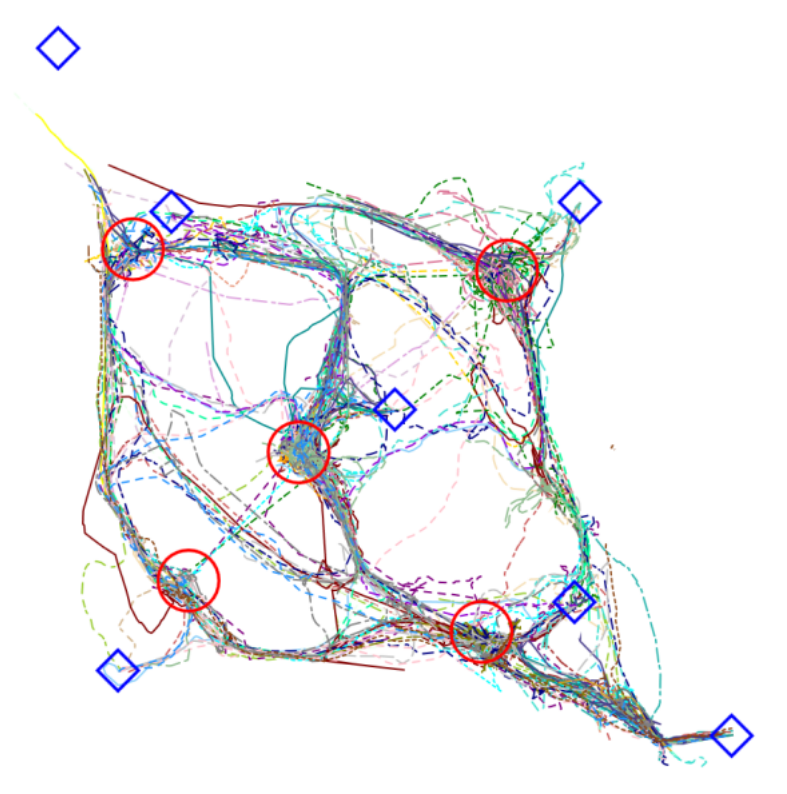
\includegraphics[width=0.9\linewidth]{Heatmap3.png}
    \caption{980 player trajectories from the ``Arathi Basin'' battleground from the game \textit{World of Warcraft}. Red circles show strategic points and blue diamonds show graveyards which are used as spawn locations. Image sourced from \cite{miller2009avatar}.}
    \label{fig:hm3}
\end{figure}

\begin{figure}[h]
    \centering
    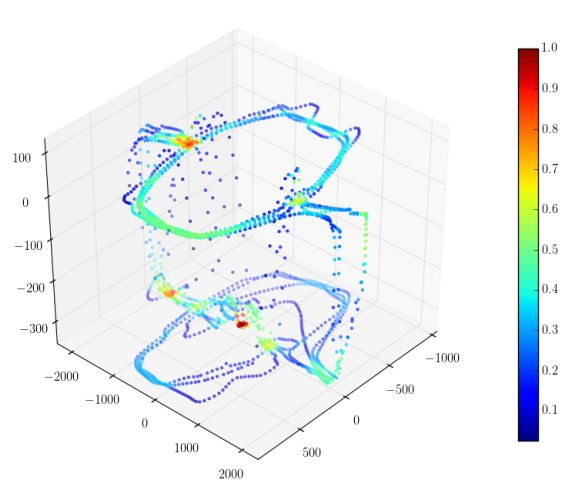
\includegraphics[width=0.8\linewidth]{Heatmap2.png}
    \caption{Representing spatial clustering and player movement in the ``Gael'' map from the game \textit{Unreal Tournament 2003}. Red areas show clustering behaviour. Image sourced from \cite{bauckhage2014beyond}.}
    \label{fig:hm2}
\end{figure}


\section{Evaluation}

The literature shows a broad approach to the trade off between network latency implications and accurately representing every entity's behaviour. Finding the balance between excessive network congestion and maintaining an accurate representation of the game state for all clients is a challenge faced by all networked multiplayer games. Dead reckoning methods are highly effective, but are solely concerned with an entity's predictable motion. Derivatives such as AntReckoning attempt to model a player's likely intention, although extending this player modelling to guide a bot representation can be rife with inaccuracy. It is apparent that where an assumption of a player's actions are incorrectly predicted, rolling back the game state can be a jarring and detrimental experience to the users.

Where network latency would cause the received data to be slightly behind, client side prediction algorithms like dead reckoning can prolong the interval of message transmissions and abolish the network latency at the cost of data consistency. In the case of lost packets resulting in no update data for that agent, client side prediction methods can be used to simulate an agent's behaviour reducing the impact of a network transmission delay. When used effectively this can help to synchronise the game state across all clients.

Related work seeks to minimise the number of required updates and maintain an up to date game state for all clients despite network latency and jitter. However, since the DIS was adopted as an IEEE standard in 1998, network bandwidth has increased considerably. This paper proposes that less strict measures be taken to reduce network load, contrasting the approaches of current methods. This paper encourages increasing the rate of network updates to be sent by dynamically altering the acceptance threshold of the client side prediction method when an entity is in a critical location in a game. Altering the threshold has been explored before, as has location evaluation in the form of interest modelling or by area of interest, but to this paper's knowledge no study has combined altering this threshold amount by a predetermined vector map showing locations where changes in motion are most unpredictable.

Furthermore, changes in acceleration shown to be common in the entity's location (consider in a racing game, a player will slow down before a corner \cite{larsson2016movement}) can be combined with the last known acceleration value in the second order projection of motion ($C.$ (2)) in a similar manner to how AntReckoning combines attraction forces. This will attempt to preempt changes in acceleration in the direction suggested by the vector map.

Unfavourable reactions from users about poor game state management show the importance of finding an effective solution to minimising client side prediction error and forms the motivation for this project. While the focus of this project is on first person shooter games, any improvement to client side prediction accuracy will be applicable to other networked multiplayer games that rely upon client side predicton and dead reckoning to maintain an up to date state representation for all clients such as racing or sports games. Given that there has been opportunity to collect information on the level layout beforehand.

\section{Methodology}

It can take some time to get used to controlling an entity in a first person shooter. 

\subsection{Hypothesis}


	\subsection{Hypotheses:} \label{hypothesis}
	\begin{table*}[h]
		\centering
		\caption{Hypotheses}
		\label{table:Hypothesis}
		\def\arraystretch{1.5}
		\begin{tabular}{|c|p{7cm}|p{7cm}|p{1.75cm}|}
			\hline
			& \textbf{Hypothesis}& \textbf{Null Hypothesis} & \textbf{Data Collection Source} \\ \hline
			%
			1 & Using bot behaviour in a level to build a vector map of aggregate changes in motion will form a representation of that level.
			& Not that.
			& Game Data \\ \hline
			%
			1 & Using bot behaviour in a level to build a vector map of aggregate changes in motion will form a representation of that level.
			& Not that.
			& Game Data \\ \hline
			
		\end{tabular}
	\end{table*}
	Table~\ref{table:Hypothesis} shows the hypotheses that are tested in this experiment. The methodologies that are used to test these hypotheses are play-testing and a questionnaire. As this required human participants for both parts ethics approval for this methodology was gained from Falmouth University’s Research Ethics Board.
	

\subsection{Participants}


% references section

\bibliographystyle{IEEEtran}
\bibliography{references}

% Appendices

%\appendices
%\section{First appendix}
%Appendices are optional. Delete or comment out this part if you do not need them.

% that's all folks
\end{document}



All participants who went outside of the track 9 or more times during the 9 laps
(not including the warm up lap) were excluded from the experiment. This resulted
in 3 out of the 26 participants being excluded. The reason why very poor
drivers were excluded was to not introduce noise into the statistics or include
data from some one who wanted disrupt the experiment on purpose.
Some of the fastest laps were completed in just over 16 seconds and some of
the slowest, in about 30 seconds. It could have been good to also set a limit on
how long a race was allowed to take before it was excluded. However, the slowest
laps were already excluded because of the first criteria. Since no participant was
observed deliberately driving slow or taking breaks during the experiment, a time
limit was never introduced.

As a reference to see how great the distances error would be if no prediction
was performed, an algorithm that did not do any updates or prediction was
implemented. The data read from the outdated node is simply passed on as the
predicted position.

This method takes the outdated position and adds the velocity multiplied by the
latency. This way a linear prediction is made.



Leading a shooting mechanic to account for lag \cite{bernier2001latency}


Describe state of field in relation to literature

Define the problem, grey lit for dead man can shoot gamasutra etc

find papers and authors that support the position I'm taking.



practical motivation

Academic motivation

Gaps in literature
Dead reckoning algorithms only use information on the player's current and simulated location and velocity.

tunnelling problem
co cognition
bots but intent needs to be carried across



what is dr

why have dr

how when where

What is good about it 
What problems does it solve
strengths

What is bad about it
weaknesses
is it a problem

propose solution